\chapter{Verification of \glsentrytext{bosss} for Inviscid Flows}
	\label{eulerVerification}
	In the following chapter we will regard a flow at Mach $0.2$ around a frictionless cylinder with adiabatic slip walls at changing parameters.
	We will compute a domain with  $-40 \leq x \leq 40$, $0 \leq y \leq 40$, a cylinder radius of $r = 1$ and the consequential level set $\varphi = x^2 + y^2 -1$. We are only considering the upper half of the domain as we can assume a symmetric flow. \\ \indent
	
	For we will regard an isentropic inviscid flow with 
	\begin{align}
			\dfrac{p}{\rho^\gamma} &= \text{const}
	\end{align}
	we can compare our results for the entropy to the analytical solution $s = 0$. Using this comparison we aim at verifying \gls{bosss} for inviscid flows and \gls{ibm}s considering robustness and convergence.
	
	\section{Robustness Study}
	In the first study regarding the frictionless cylinder, we compare the absolute error of entropy for a polynomial degree from $1$ to $3$ along a shift of the centre point of the cylinder from $-0.075$ to $0.075$ at steps of $0.015$. Therefore the level set $\varphi$ will now be described by $\varphi = x^2 + y^2 - (1+ \text{shift})^2$. By shifting the cylinder we can consider several cases where the cells would be cut differently and therefore cause different cell agglomerations. The cell agglomeration threshold is at a constant level of $0.5$ in a mesh of $64 \times 64$ cells (see \cref{fig:eulershift}) thus causing different cell agglomerations with every shift. In this example we aim at proving the robustness of the solver as for each position of the cylinder the error of entropy should not vary too much thus making it independent of the way the border cells are cut. \\ \\

	\begin{figure}[htp]	
		\centering
		\begin{tikzpicture}
			\begin{semilogyaxis}[xlabel ={Position of Centre Point of the Cylinder}, ylabel ={$L_2$ Error of Entropy}, grid =major, legend entries ={$P=1$,$P=2$, $P=3$}, unbounded coords=jump, legend style = {cells = {anchor=east}, legend pos=outer north east,}, scaled x ticks = false]
				\addplot table[ x =shift, y =error1] {data/shift.dat};
				\addplot table[ x =shift, y =error2] {data/shift.dat};
				\addplot table[ x =shift, y =error3] {data/shift.dat};
			\end{semilogyaxis}	
		\end{tikzpicture}
		\caption{Convergence Plot}
		\label{shifterror}
	\end{figure}
	

	As we look at \cref{shifterror}, first of all we will note that the absolute error of entropy decreases with increasing polynomial degree. As a higher polynomial degree implies a better approximation this can be explained very easily. \\ \indent
	Secondly, we can observe that the error of entropy behaves roughly symmetrically to the ordinate which is unsurprising as we shifted the cylinder symmetrically.\\ \indent
	For degree 1 and 2 the error is at a fairly constant value throughout the cylinder shift; at the polynomial degree 3 it is very irregular. The two most discordant values appear at a shift of $\pm 0.03$. There the calculation was very unstable. By varying the parameters explained in \cref{parameters} we made them as stable as possible but still produced the inaccurate values shown in \cref{shifterror}. \\ \indent
	We can therefore infer that with increasing polynomial degree at a mesh that course the calculation gets very unstable; a finer mesh should be used. \\ \indent
	Now we will consider two cases which have the largest error difference apart from degree 3 - degree $2$ at the shifts $-0.06$ and $-0.03$ - more closely. \\\\
	
	\begin{figure}[htp]
		\centering
		\begin{minipage}[b]{0.5\textwidth}
			\centering
			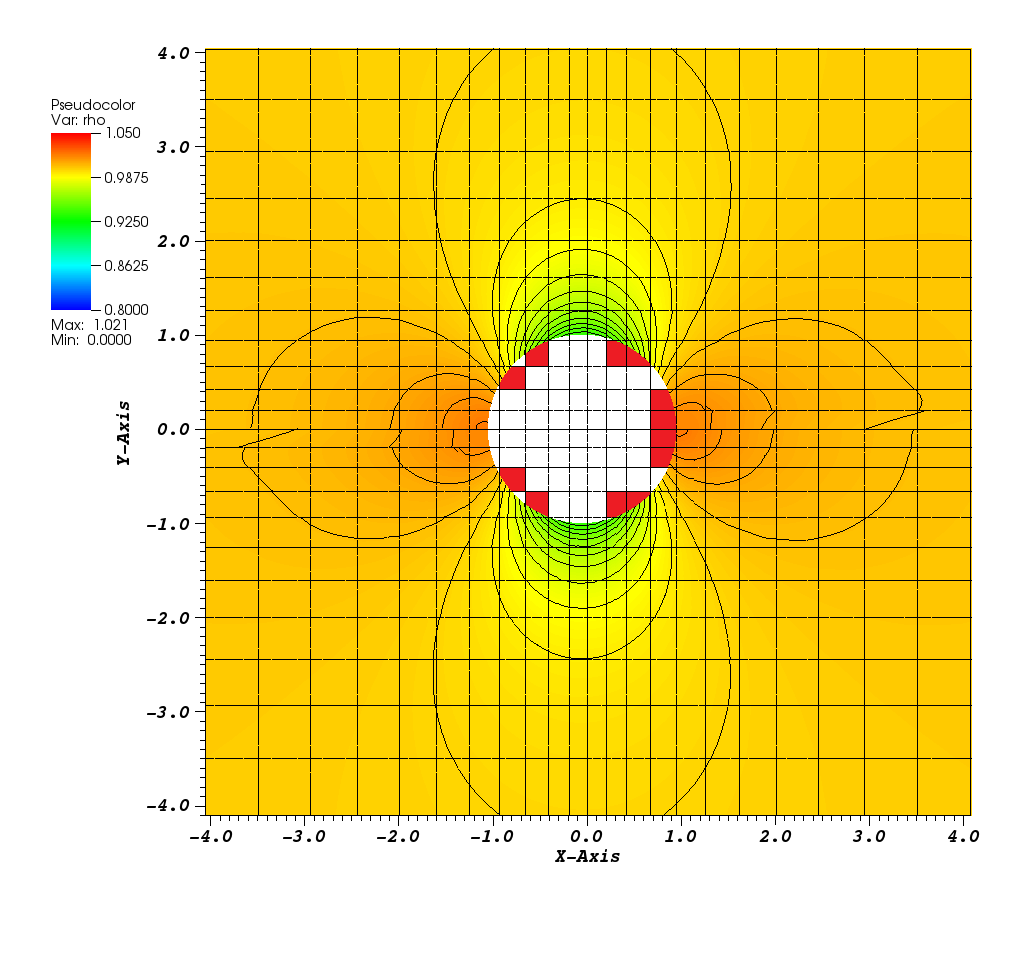
\includegraphics[height=8cm]{2_2.png}
			\caption*{Degree 2, shift $-0.06$}
			\label{fig:2_2}
		\end{minipage}%
		\begin{minipage}[b]{0.5\textwidth}
			\centering
			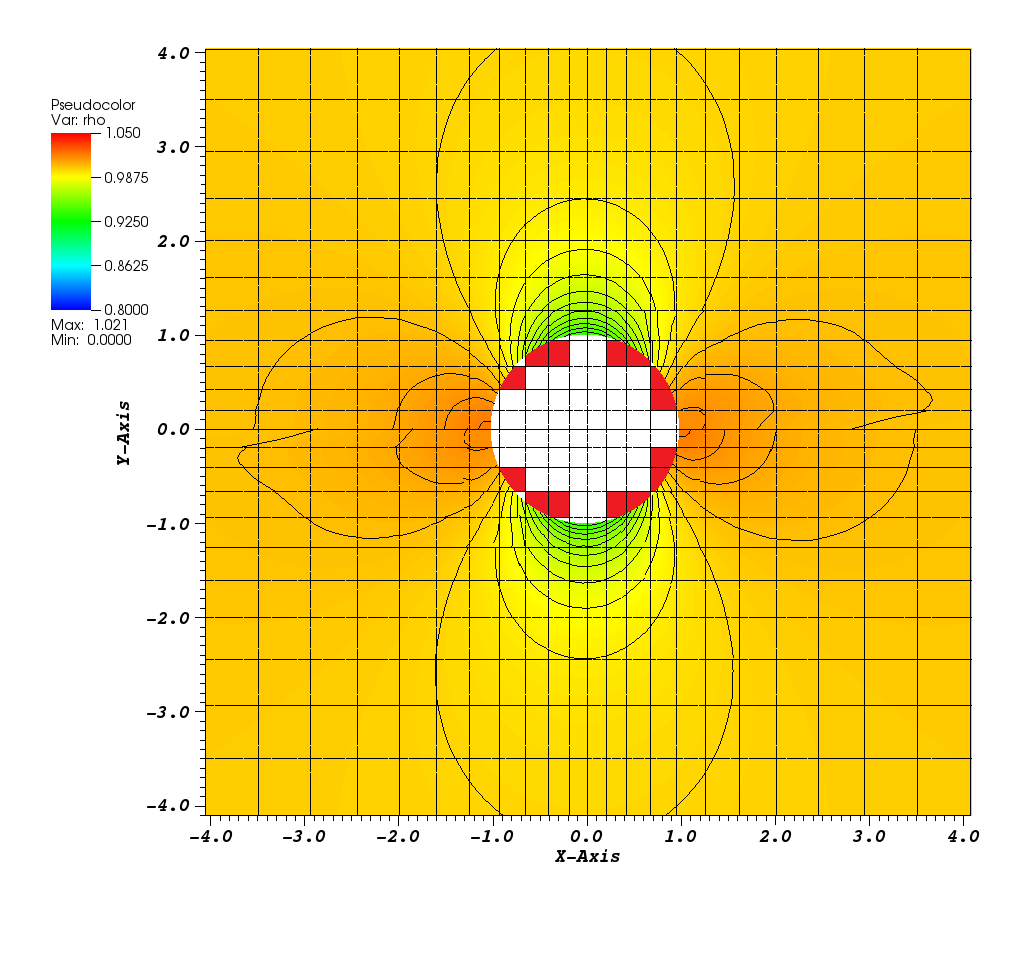
\includegraphics[height=8cm]{2_4.png}
			\caption*{Degree 2, shift $-0.03$}
			\label{fig:2_4}
		\end{minipage}
		\caption{Isolines of pressure}\label{fig:isoshift}
	\end{figure}
	
	In \cref{fig:isoshift} you can see the two mentioned cases with highlighted isolines of pressure and pseudocoloured density. As only the upper half of the cylinder has been calculated, we reflected the results through the centre point of the cylinder. Therefore you can easily see that the results are not flawless, as the flow before and after the obstacle should be identical. Furthermore you can see that in the left picture the isolines are smoother than in the right one. We also highlighted the cells that have been agglomerated in red; in the right case almost every cut cell has been agglomerated while in the left one it were fewer. It may be assumed, that each agglomeration causes an error which results into the higher error that we remarked in \cref{shifterror}. Unfortunately we did not find a proper explanation for the agglomeration error; this could be subject of future research. \\\\ 
	
	Except for the polynomial degree $3$, the error of entropy changes very little for the different cases. We can therefore assume that the solver is good enough validated concerning the way the agglomerated cells influence the calculation as long as we consider a fine enough mesh for higher degrees.
	
	\section{Convergence Study of Mesh Size and Polynomial Degree}
	
	In the second study we vary the mesh size of our geometry from $32 \times 32$ by $64 \times 64$ to $128 \times 128$ cells. Additionally we also vary the polynomial degree from $0$ to $4$, consequently regarding fifteen cases in total. The agglomeration factor is at a constant moderate level $\alpha = 0.3$.\\
	Our aim is the validation of the convergence of the \gls{rkdg} method based solver for the inviscid cylinder. Therefore we hope to achieve an experimental order of convergence that is near the optimal rate $O(h^{P+1})$. In  \cref{mesherror} we compared the absolute error entropy to the mesh size logarithmically for each polynomial degree and added the linear regressions $R_P$ with its slopes to each graph. 	\\\\
	\begin{figure}[htp]
		\centering		
		\begin{tikzpicture}
			\begin{loglogaxis}[xlabel ={Cells per Direction}, ylabel ={$L_2$ Error of Entropy}, grid =major, legend entries ={$P=0$,$P=1$,$P=2$, $P=3$, $P=4$, $R_0$, $R_1$, $R_2$, $R_3$, $R_4$}, unbounded coords=jump, legend style = {cells = {anchor=east}, legend pos=outer north east,} ]
				\addplot table[ x =meshSize, y =error0] {data/test.dat};
				\addplot table[ x =meshSize, y =error1] {data/test.dat};
				\addplot table[ x =meshSize, y =error2] {data/test.dat};
				\addplot table[ x =meshSize, y =error3] {data/test.dat};
				\addplot table[ x =meshSize, y =error4] {data/test.dat};
				\addplot table[
				x=meshSize,
				y={create col/linear regression={						y=error0,}}	]
				{data/test.dat}
				coordinate[pos=0.6] (A)
				coordinate[pos=0.75] (B);
				\xdef\nullslope{\pgfplotstableregressiona}
				\draw (A) -| (B)
				node [pos=0.75, anchor = south west] {\pgfmathprintnumber[fixed]{\nullslope}};
				\addplot table[
				x=meshSize,
				y={create col/linear regression={						y=error1,}}	]
				{data/test.dat}
				coordinate[pos=0.6] (A)
				coordinate[pos=0.75] (B);
				\xdef\einsslope{\pgfplotstableregressiona}
				\draw (A) -| (B)
				node [pos=0.75, anchor = west] {\pgfmathprintnumber{\einsslope}};
				\addplot table[
				x=meshSize,
				y={create col/linear regression={						y=error2,}}	]
				{data/test.dat}
				coordinate[pos=0.6] (A)
				coordinate[pos=0.75] (B);
				\xdef\zweislope{\pgfplotstableregressiona}
				\draw (A) -| (B)
				node [pos=0.75, anchor = west] {\pgfmathprintnumber{\zweislope}};
				\addplot table[
				x=meshSize,
				y={create col/linear regression={						y=error3,}}	]
				{data/test.dat}
				coordinate[pos=0.6] (A)
				coordinate[pos=0.75] (B);
				\xdef\dreislope{\pgfplotstableregressiona}
				\draw (A) -| (B)
				node [pos=0.75, anchor = west] {\pgfmathprintnumber{\dreislope}};
				\addplot table[
				x=meshSize,
				y={create col/linear regression={						y=error4,}}	]
				{data/test.dat}
				coordinate[pos=0.6] (A)
				coordinate[pos=0.75] (B);
				\xdef\vierslope{\pgfplotstableregressiona}
				\draw (A) -| (B)
				node [pos=0.75, anchor = west] {\pgfmathprintnumber{\vierslope}};
			\end{loglogaxis}	
		\end{tikzpicture}	
		\caption{Convergence Plot}
		\label{mesherror}
	\end{figure}
	
	As you can see in \cref{mesherror} each graph has a quite constant slop that is higher with increasing polynomial degree. For $1 < P < 4$ it is approximately of the order $P+1$ as we hoped, only for $P = 0$ the computations converge much more slowly.\\ \indent
	Again it was necessary to adjust some of the parameters explained in \cref{parameters} in order to stabilise the calculations with higher polynomial degrees. \\ \indent
	As an example for the correction of a critical calculation we visualised the case with mesh size $128 \times 128$ and polynomial degree $P = 3$ before and after the correction in \cref{fig:case14}. Again, we visualised entropy and pressure. The picture in the middle shows a zoomed view of the critical cell where a high amount of entropy was produced and lead to the breakup. Please remark that differently coloured entropy ranges had to be used before and after the correction in order to point out the critical cell.
	\begin{figure}[htp]
		\centering
		\begin{minipage}[b]{0.3\textwidth}
			\centering
			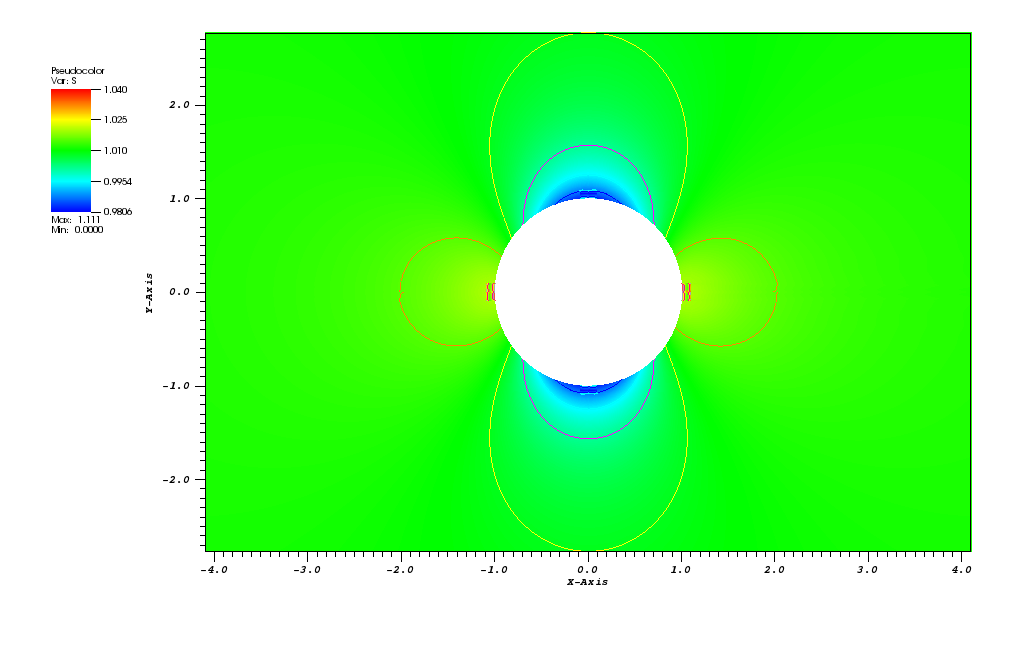
\includegraphics[height=3.8cm]{img/case14.png}
			\caption*{Overview of flow before correction}
		%	\label{fig:case14gross}
		\end{minipage}
		\quad
		\begin{minipage}[b]{0.3\textwidth}
			\centering
			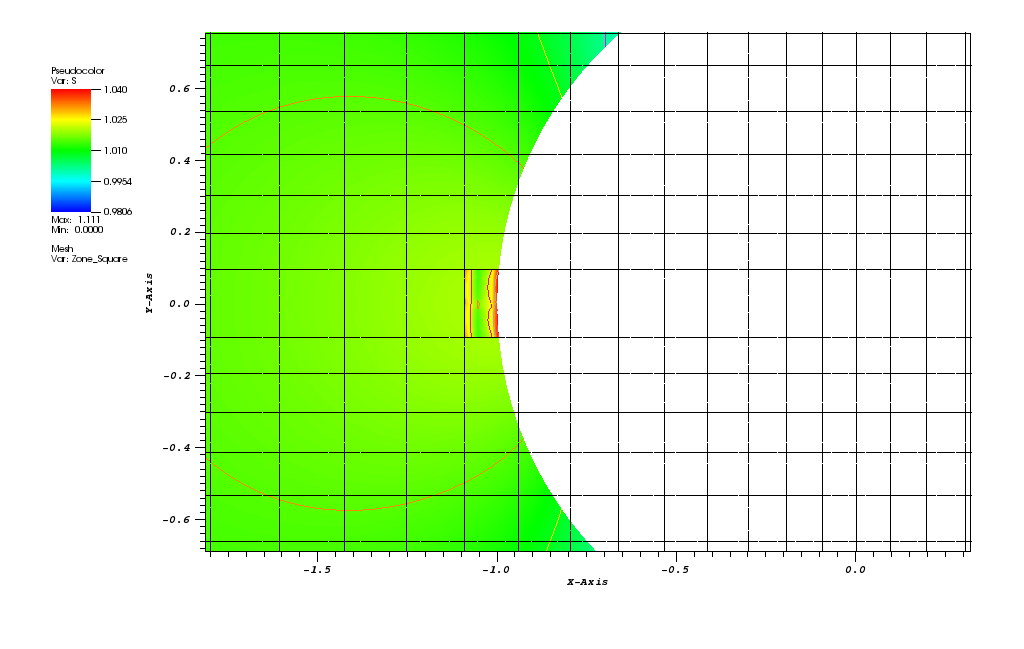
\includegraphics[height=3.8cm]{case14komisch.png}
			\caption*{Detailed view of critical cell before correction}
			\label{fig:case14detail}
		\end{minipage}
		\quad
		\begin{minipage}[b]{0.3\textwidth}
			\centering
			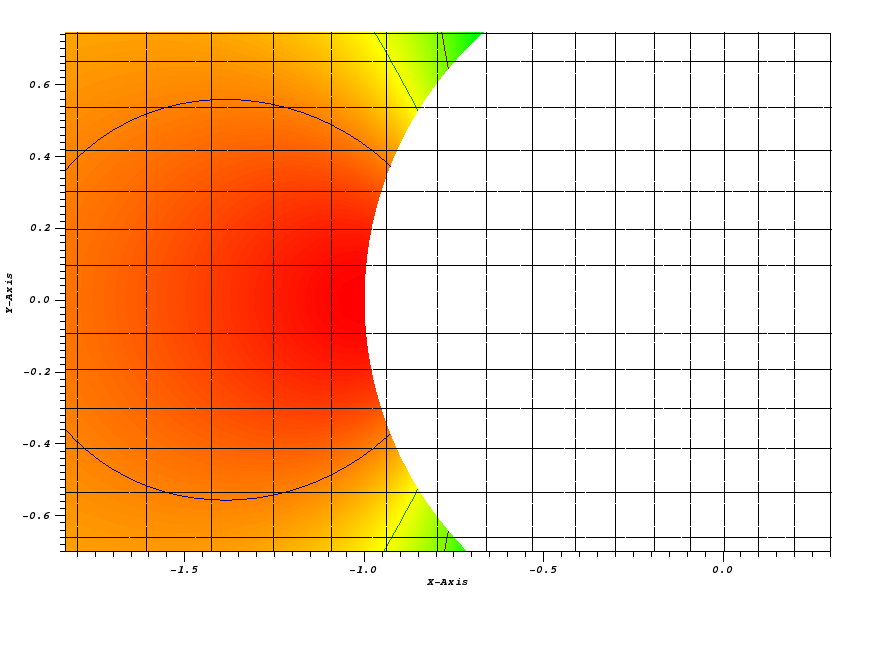
\includegraphics[height=3.8cm]{case14normal.png}
			\caption*{Detailed view of critical cell after correction}
			\label{fig:case14detailneu}
		\end{minipage}
		\caption{Mesh size $128 \times 128$, $P = 3$}
		\label{fig:case14}
	\end{figure}
	
	\section{Conclusion}
	
	After having studied the behaviour of \gls{bosss} concerning the Euler equations with immersed boundaries, we can conclude that is sufficiently validated. The robustness studied showed that the results are mostly independent from the exact position of the grid cells. During the convergence study we remarked  that the convergence behaves as desired with an order close to the optimal rate of $O(h^{P+1})$. 
	
	Nevertheless in order to receive the correct results one sometimes needs to put a large effort into adjusting parameters for stable calculations. 